\section{Introduction} % Pas de numérotation
\addcontentsline{toc}{section}{Introduction} % Ajout dans la table des matières
 \subsection{Introduction du CMCC}
Le 3 avril 1973, M. Mation \textsc{cooper} le directeur général de la division communication de Motorola, à effectuer un appel téléphonique à Joel \textsc{engel}, son rival et néanmoins confrère chez \textsf{Belle Labs}. c'est la premier appel téléphonique en extérieur, L'idée du téléphone portable devient une réalité. 


depuis ce jour, le technique développé très rapidement. dans les 20 dernières années, il y a déjà quatre génération des standards pour la téléphonie mobile, non seulement nous pouvons appeler les autres, les nouvelles technologies et les Smart-phones nous permettons aussi envoyer les message, surfer l'Internet, utiliser le service RTSP(Real Timide Streaming Protocol), et le service VoIP (Voice over Internet Protocole),etc.. les services de communication téléphonique sont devenus un outil très important dans notre vie.
 
 
Fondé en 3 Septembre 1997, après le regroupement de opérateur des télécommunications en 2008, \textsc{China Mobile Communications Corp.} (\textsf{CMCC})\ref{Fig.sub.1} est devenu un de trois opérateur des télécommunications en Chine (deux autres sont \textsf{China Unicom Co., Ltd.} et \textsf{China Telecom}). Après plusieurs années de développement, il a construit le plus grand réseau de communications mobiles dans le monde, possède la plus grande base d'utilisateurs dans le monde\ref{Fig.sub.2}. En 2013, CMCC a 767 million utilisateurs, 630,2 billion\textyen de revenu, 121,7 billions \textyen de revenus net, effectif 197,030.
\begin{figure}[H]
	\flushleft
	\subfigure[Logo de China Mobile]{
		\label{Fig.sub.1}
		
\includegraphics[width=1.8in]{images/China_Mobile_2013.png}}\hfill
	\hspace{1in}
%\flushright
	\subfigure[Reseau télécommunication]{
		\label{Fig.sub.2}
		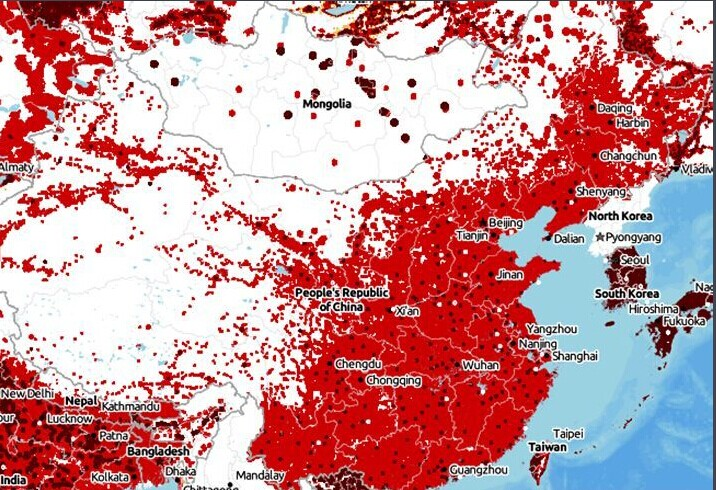
\includegraphics[width=2.0in]{images/reseau.jpg}}
	\caption{CMCC} 
\end{figure}


Mais en même tempe, le taux de croissance des nouveaux utilisateur décline de 22,5 \% (2006) à moins de 5\% 2013. Et dans la premier 3 mois, l'entreprise une fois considérés comme \href{http://www.marketing-chine.com/entreprises-chinoises/le-top-50-des-marques-chinoises}{la plus rentable de Chine}, le taux de croissance des revenu net est 0,3\%.

Les données fournies par Vodafone montre que lorsque la mise è niveau du réseau mobile de 2G à 3G, utilisateur utilise moins de service vocaux, en même temps ils utilisent plus les services internet, et le ARPU (Average Revenue Per User) total décline aussi \ref{vodafone1}. En utilisant les nouvelles technologies (2G/3G/4G), les utilisateurs utilisent plus souvent le service internet.
 \begin{figure}[H]
 	\flushleft
 	\subfigure[étude de Vodafone]{
 		\label{vodafone1}
 		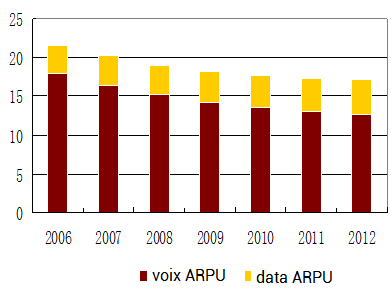
\includegraphics[width=1.8in]{images/2.png}}\hfill
 	\hspace{1in}
 %\flushright
 	\subfigure[Downlink Data Traffic in 2G/3G Network]{
 		\label{vodafone2}
 		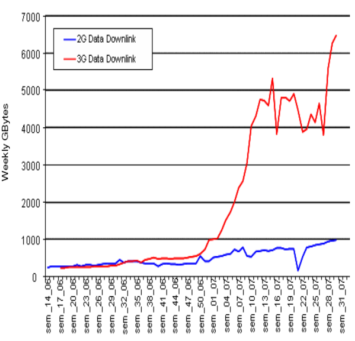
\includegraphics[width=2.0in]{images/4.png}}
 	\caption{Vodafone} 
 \end{figure}
   
 
  
  
  
\subsection{Introduction du laboratoire}
 %从1876年贝尔发明电话至今,已经有100多年的历史。目前电话通信服务已成为人们交流信息不可或缺的重要工具。最近20年来,
 %从模拟到数字、从单频到双频、从英文菜单到中文输入、从语音到短信,新的技术和业务不断推出
 De 20 Avril 2014 à 20 Juillet 2014, je fait mon stage chez \href{http://203.91.121.76/joomla/}{laboratoire of Next Generation Network Technology \& Application} \textsf{( NGN )} \ref{Logo NGN}. C'est d'un subordonné de \href{http://www.ee.tsinghua.edu.cn/publish/eeen/3776/index.html}{Research Institute of Network And Human-Machine Speech Comunication}, Département Ingénierie électronique, Tsinghua University. Le laboratoire se trouve dans la ROHM bâtiment.
  \begin{figure}[H]
      \centering
      
\includegraphics[width=3in]{images/NGN.jpg}
      \caption{Logo NGN}
      \label{Logo NGN}
  \end{figure}
Le principaux axes de recherche sont Théorie des réseaux, Architecture de l'Internet, Traitement de l'information Internet, La recherche dans le domaine de la sécurité Internet, Sentiment analyse, Information hiding, etc.

 Mon tuteur professionnel est \href{http://203.91.121.76/joomla/index.php/staff/teacher/83-huangyongfeng}{M. Yongfeng \textsc{huang}}, vice-directeur de la laboratoire NGN. Dans le laboratoire, il y a cinq groupe, dans notre groupes, il y a un docteur, une master .







%\begin{figure}[P]
%	\flushleft
%	\subfigure[Logo de China Mobile]{
%		\label{Fig.sub.1}
%		
\includegraphics[width=1.8in]{images/China_Mobile_2013.png}}\hfill
%	\hspace{1in}
%\flushright
%	\subfigure[Reseau télécommunication]{
%		\label{Fig.sub.2}
%		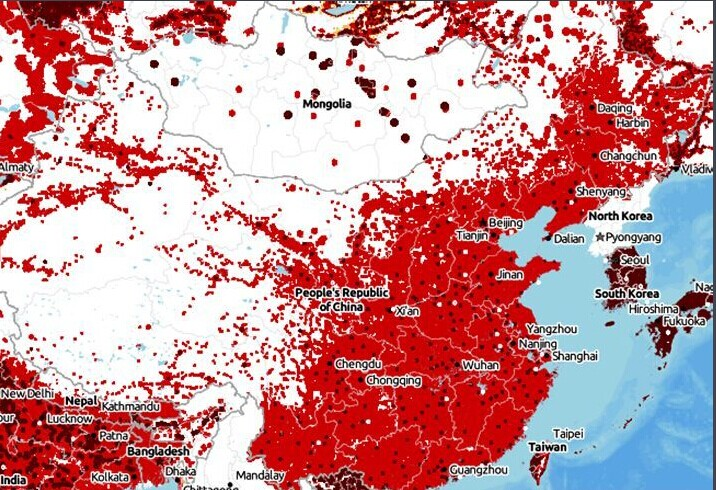
\includegraphics[width=2.0in]{images/reseau.jpg}}
%	\caption{CMCC} 
%	\label{Fig.1}
%\end{figure}


%\begin{figure} 
%  \centering 
%  \subfigure[Small Box with a Long Caption]{ 
%    \label{fig:subfig:a} %% label for first subfigure 
%    
\includegraphics[width=1.5in]{images/China_Mobile_2013.png}} 
% \hspace{1in} 
%  \subfigure[Big Box]{ 
%    \label{fig:subfig:b} %% label for second subfigure 
%    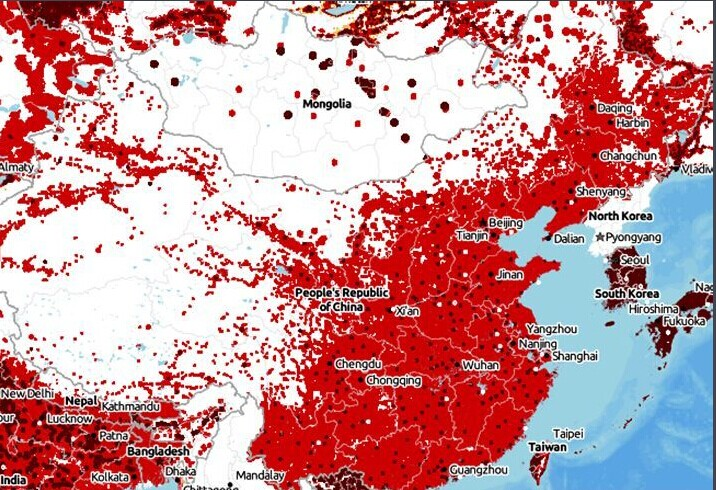
\includegraphics[width=1.5in]{images/reseau.jpg}} 
%  \caption{Two Subfigures} 
%  \label{fig:subfig} %% label for entire figure 
%\end{figure}


Ce document est un exemple de rapport. J'espère aider des étudiants à réaliser leur rapport en \LaTeX.

Écrit par Bruno Voisin (Hiko Sejûrô) et publié sur \url{http://blog.hikoweb.net/}.

%\begin{figure}[!ht]
%    \center
%    
\includegraphics[]{images/China_Mobile_2013.png}
%    \caption{Logo China Mobile}
%    \label{ChinaMobile}
%\end{figure}

%\begin{figure}[!ht]
%    \center
%    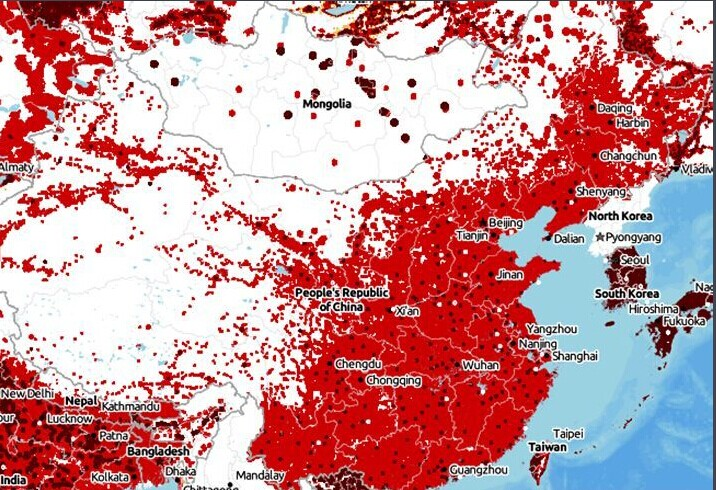
\includegraphics[]{images/reseau.jpg}
%    \caption{Réseau télécommunication en Chine}
%    \label{Reseau}
%\end{figure}